\documentclass[11pt,a4paper]{article}
\usepackage[a4paper,hmargin=1in,vmargin=1in]{geometry}
\usepackage{pgfplots}
\pgfplotsset{compat=1.17}

\usepackage[british]{babel}
\usepackage[utf8]{inputenc}
\usepackage[T1]{fontenc}

\usepackage[nodayofweek]{datetime}
\newdate{Date}{26}{1}{2024}

\usepackage{stddoc}

\def\MHz{\,\mathrm{MHz}}
\def\Hz{\,\mathrm{Hz}}


\begin{document}

    \pagenumbering{arabic}

    % Header
    \begin{center}
        {\LARGE\textbf{B2M34NSV - Semester project}}\\[3mm]
        \begin{minipage}{0.4\textwidth}
            \begin{flushleft}
                \textsc{\displaydate{Date}}
            \end{flushleft}
        \end{minipage}
        ~
        \begin{minipage}{0.4\textwidth}
            \begin{flushright}
                \textsc{Martin Šimák}
            \end{flushright}
        \end{minipage}
        \noindent\rule{14.5cm}{0.4pt}
    \end{center}

    \paragraph{Task} \emph{Brownian motion of molecules displayed using a VGA interface}
    The project aim was to implement a Brownian thermal motion of a molecule or another small particle (pollen grain) which is then displayed as a ball on a monitor using a VGA interface. The program runs on a development board Basys 3 designed by Digilent. The Basys 3 is built around the Xilinx Artix-7 FPGA which is a programmable logic device, preferably worked with using the Vivado software suite.

    \subsection*{General description}
        \paragraph{Controls} The program requires no interaction, and it works autonomously immediately after programming the device. However, there are three possible manipulation controls:
        \begin{itemize}
            \item The centre button (\emph{BTNC}) works as a reset button which can be utilized to restore the default position of the balls.
            \item The first two switches (\emph{SW0} and \emph{SW1}) control the random generation of balls movement direction. The first switch controls the first, faster ball and the second switch controls the second, slower ball.
        \end{itemize}

        The whole system schematic can be seen in Figure~\ref{fig:schematic}. Furthermore, the device resources allocation is illustrated in Figure~\ref{fig:device}.

    \subsection*{Modules}
        Below are listed all the modules making up the whole system. It is worth noting that apart from the inputs and outputs, the VHDL design was performed using generics allowing for the parametrization of the whole system. This way it is easy to change various parameters such as the radii of the balls, the dimensions of the used monitor (in pixels) and the encompassing frame width (in pixels).

        \subsubsection*{Top-level hierarchy module}
            The top level entity connects all the inner components together and is responsible for their proper connection. The output signals are standard signals controlling the VGA display.\\[1em]
            \emph{Inputs:} Clock signal, reset button, two switches.\\[1em]
            \emph{Outputs:} RGB colour signals, horizontal and vertical synchronization.

        \subsubsection*{Clock divider}
        \begin{minipage}{.45\textwidth}
            \emph{Inputs:} System clock signal of frequency $100\MHz$, reset button.\\[1em]
            \emph{Outputs:} Five output clock signals of frequencies $50\MHz$, $100\Hz$, $50\Hz$, $4\Hz$ and $2\Hz$.\\[1em]
            \emph{Description:} This component serves the purpose of dividing the frequency of the system clock signal, generating five internal clock signals required by other components. Namely, the $50\MHz$ signal clocks the VGA drawing signals, the $100\Hz$ and $50\Hz$ signals clock the movement of the faster and the slower balls respectively, and the $4\Hz$ and $2\Hz$ signals clock the rate of random direction change generated by the shift registers (see below).
        \end{minipage}
        \hfill
        \begin{minipage}{.45\textwidth}
            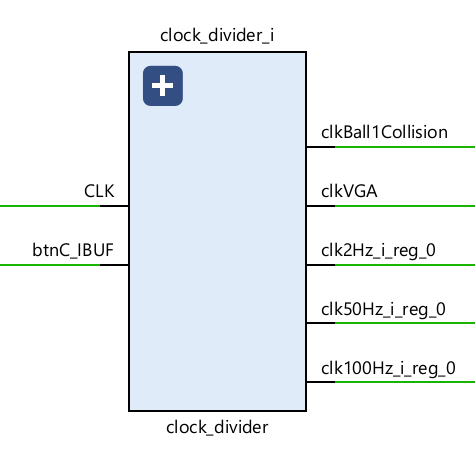
\includegraphics[width=\textwidth]{src/clock-divider.png}
        \end{minipage}

        \subsubsection*{Frame graphical component}
        \begin{minipage}{.45\textwidth}
            \emph{Inputs:} Clock signal ($50\MHz$), reset button, current drawing position coordinates.\\[1em]
            \emph{Outputs:} RGB colour signals.\\[1em]
            \emph{Description:} This component is responsible for displaying the frame encompassing the scene. It only decides whether the frame should be drawn on the current drawing position.
        \end{minipage}
        \hfill
        \begin{minipage}{.45\textwidth}
            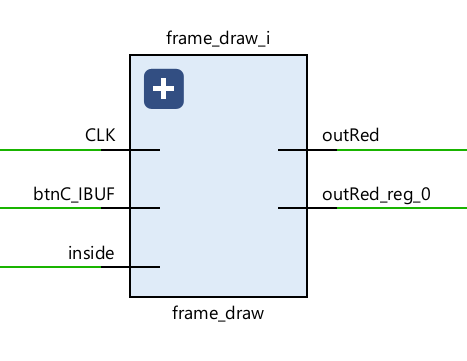
\includegraphics[width=\textwidth]{src/frame-draw.png}
        \end{minipage}

        \subsubsection*{LFSR}
        \begin{minipage}{.45\textwidth}
            \emph{Inputs:} Clock signal, reset button, enable bit.\\[1em]
            \emph{Outputs:} MSB, LSB.\\[1em]
            \emph{Description:} This component is an ordinary Linear Feedback Shift Register (LFSR) which can generate a pseudorandom sequence of bits the length of which is determined by the length and the seed of the LFSR. It is instantiated twice in the top-level module, once with a $4\Hz$ clock signal and length of 32 bits for the faster, smaller ball and second with a $2\Hz$ clock signal and length of 16 bits for the slower, larger ball. The current state MSB is further interpreted as a virtual collision indicator of the controlled ball in the $x$-direction and the LSB in the $y$-direction. This results in a very long pseudorandom sequence of direction changes mimicking the Brownian thermal motion.
        \end{minipage}
        \hfill
        \begin{minipage}{.45\textwidth}
            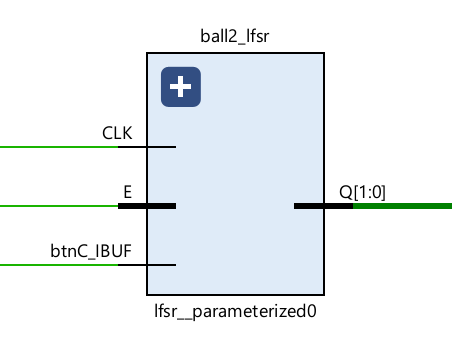
\includegraphics[width=\textwidth]{src/lfsr.png}
        \end{minipage}

        \subsubsection*{Ball movement component}
        \begin{minipage}{.45\textwidth}
            \emph{Inputs:} Clock signal, reset button, virtual collision bits in $x$ and $y$, current position coordinates of the other ball.\\[1em]
            \emph{Outputs:} Current position coordinates of the drawn ball.\\[1em]
            \emph{Description:} This component contains the logic behind the movement of a ball and is instantiated twice in the top-level module - once for each ball. The contained logic takes into account the generated pseudorandom direction changes but also deals with the collisions of the ball with the encompassing walls (drawn frame) and the balls with each other. The velocity of each ball is determined by the assigned clock signal frequency: $100\Hz$ for the faster, smaller ball and $50\Hz$ for the slower, larger ball.
        \end{minipage}
        \hfill
        \begin{minipage}{.45\textwidth}
            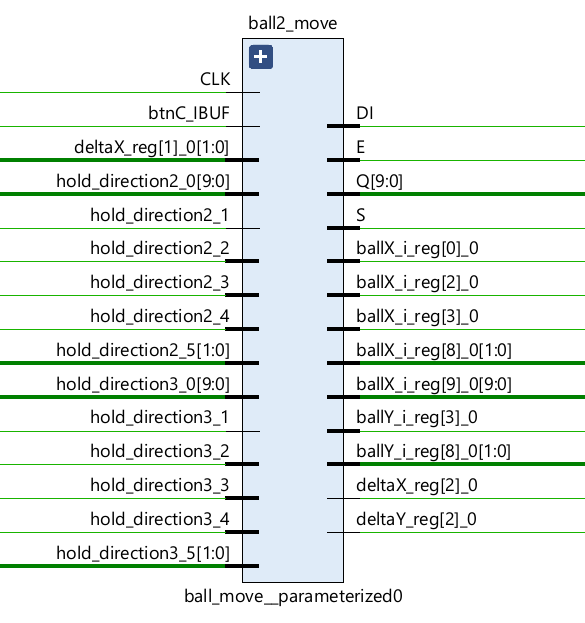
\includegraphics[width=\textwidth]{src/ball-move.png}
        \end{minipage}

        \subsubsection*{Ball graphical component}
        \begin{minipage}{.45\textwidth}
            \emph{Inputs:} Clock signal ($50\MHz$), reset button, current drawing position coordinates, current ball position coordinates.
            \emph{Outputs:} RGB colour signals.
            \emph{Description:} This component is responsible for displaying given ball. Therefore, it is also instantiated twice in the top-level module. It only decides whether the ball should be drawn on the current drawing position.
        \end{minipage}
        \hfill
        \begin{minipage}{.45\textwidth}
            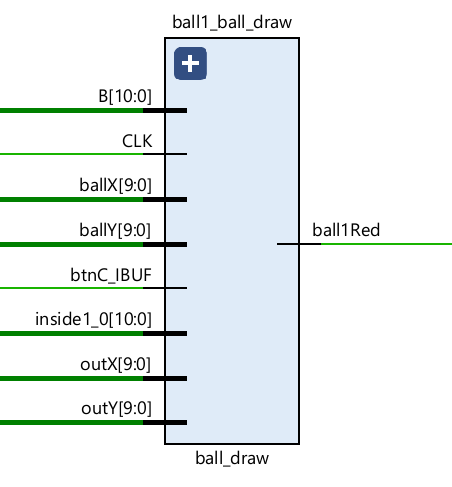
\includegraphics[width=\textwidth]{src/ball-draw.png}
        \end{minipage}

        \subsubsection*{Colour multiplexer}
        \begin{minipage}{.45\textwidth}
            \emph{Inputs:} Clock signal ($50\MHz$), reset button, RGB colour signals from three objects present in the scene.
            \emph{Outputs:} Output RGB colour signals.
            \emph{Description:} The colour multiplexer is a simple \emph{OR} performed between the passed signals per component. It basically adds up the RGB colour signals from the objects to be displayed in the scene.
        \end{minipage}
        \hfill
        \begin{minipage}{.45\textwidth}
            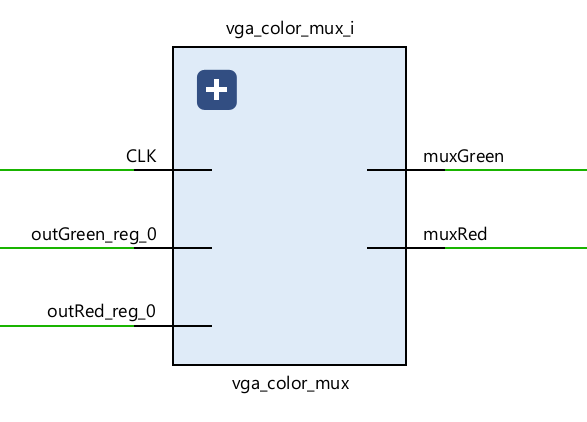
\includegraphics[width=\textwidth]{src/color-mux.png}
        \end{minipage}

        \subsubsection*{VGA signal generator}
        \begin{minipage}{.45\textwidth}
            \emph{Inputs:} Clock signal ($50\MHz$), reset button, RGB colour signals.\\[1em]
            \emph{Outputs:} Vertical and horizontal synchronization signals, VGA colour signals, current drawing position coordinates.\\[1em]
            \emph{Description:} This component is basically the VGA driver which generates the final signal which is then sent into the VGA interface. It adapts the already generated signals to adhere to the VGA interface standard.\\[1em]
            \emph{Note:} This component was mostly written by the lecturer and given to me for adaptation.
        \end{minipage}
        \hfill
        \begin{minipage}{.45\textwidth}
            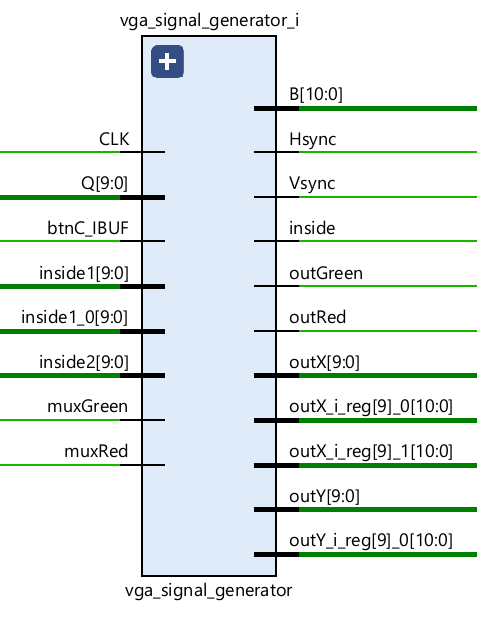
\includegraphics[width=\textwidth]{src/vga-signal-generator.png}
        \end{minipage}

    \subsection*{Conclusion}
        The final program displays two molecules moving in a pseudorandom pattern mimicking the Brownian thermal motion. The whole scene is encompassed by a frame which deflects the molecules hitting it. The project was made significantly more difficult by adding a molecule to the scene posing some challenges in terms of dealing with more complex collision detection.

        Further development can be seen in adding more variability to the scene, such as more molecules of different sizes and velocities. There are also some non-physical aspects which can be seen upon closer inspection of the deflections during collisions and which could be improved upon.




\newpage
    \subsection*{Figures}

    \begin{figure}[!ht]
        \centering
        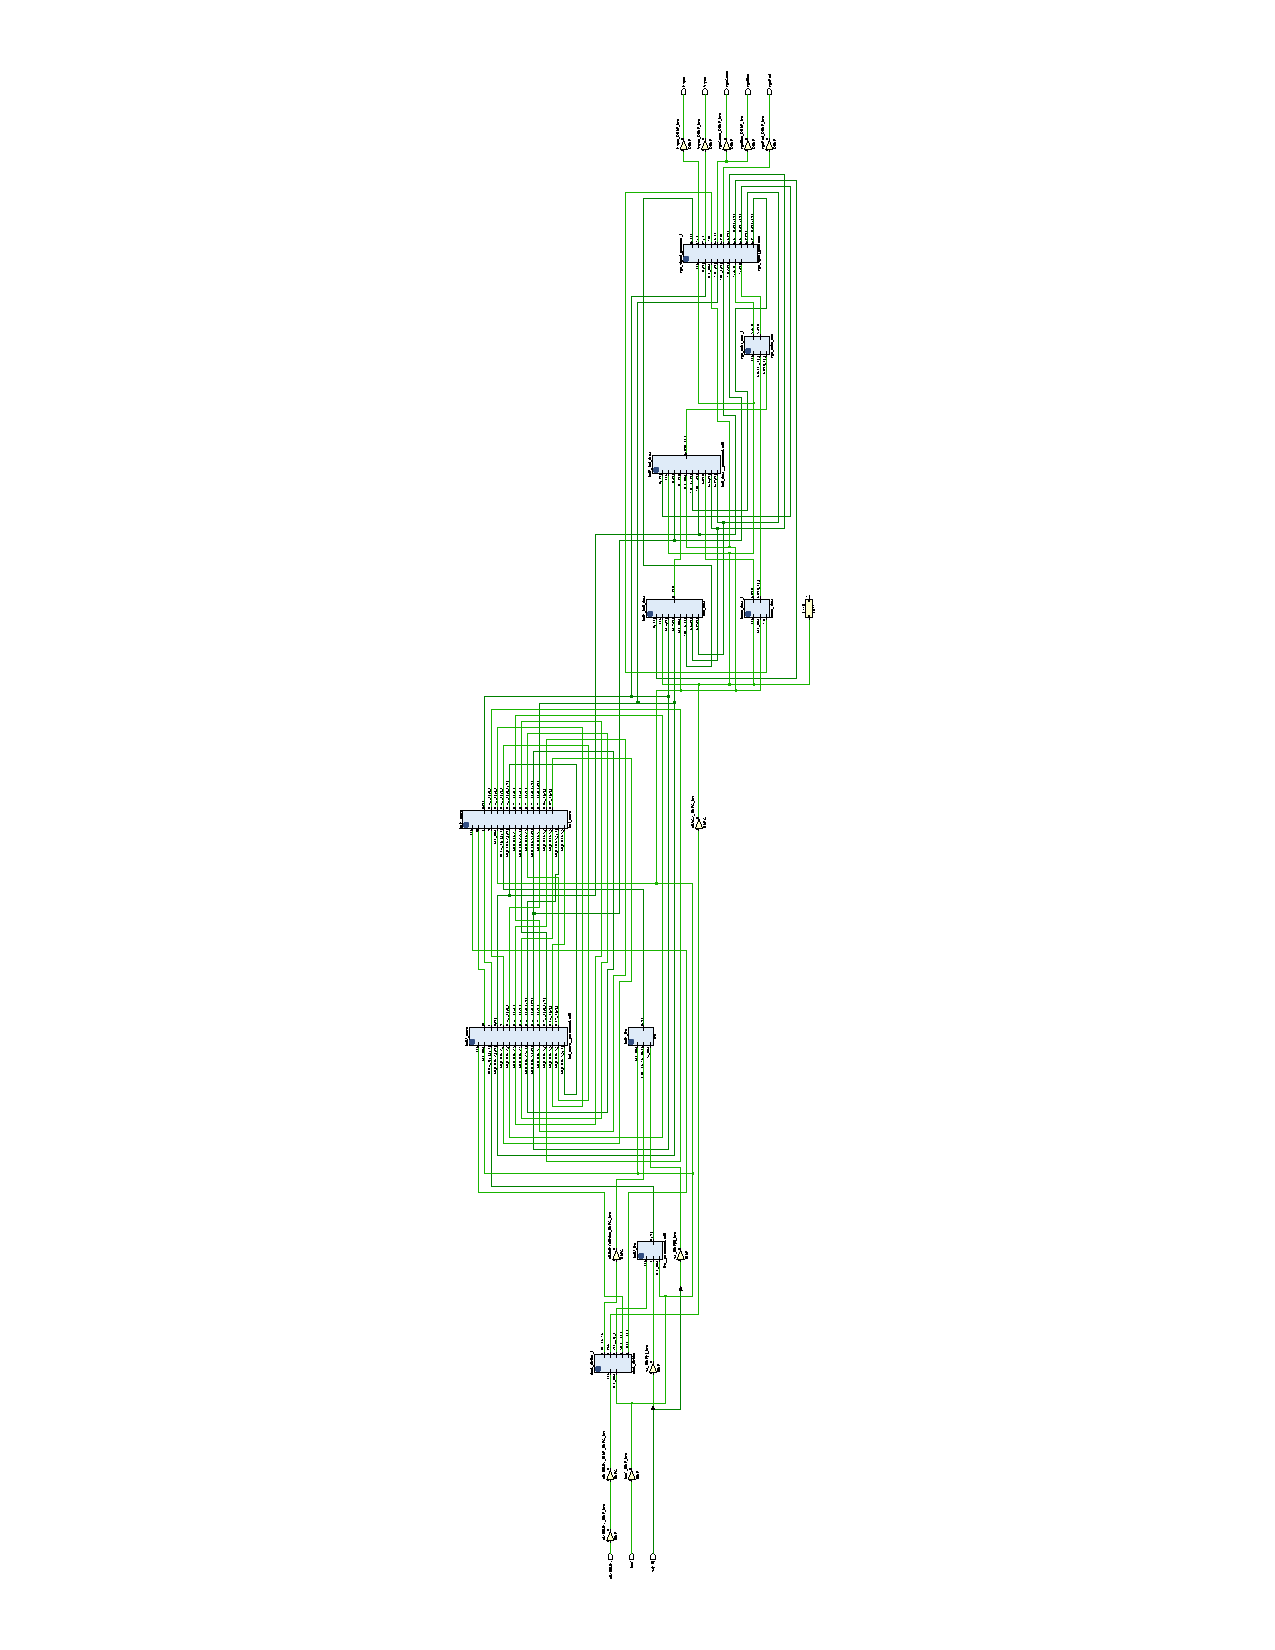
\includegraphics[width=\textwidth]{src/schematic.pdf}
        \caption{\label{fig:schematic}Digital circuit schematic}
    \end{figure}

    \begin{figure}[!ht]
        \centering
        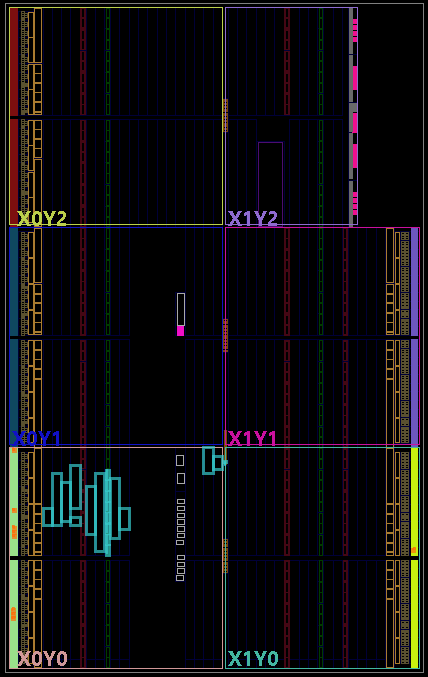
\includegraphics[width=.6\textwidth]{src/device.png}
        \caption{\label{fig:device}Device resources allocation}
    \end{figure}

\end{document}